\subsection{Discrete resistor}
The first results obtained using the impedance-sensing system is of an impedance spectroscopy for a 10 k$\Omega$ discrete resistor. Measured with an ohmmeter, its DC resistance is of 9.95 k$\Omega$. The impedance-sensing system is activated in Multi-frequency mode for a lowest excitation frequency of 20 kHz and a highest of 11.81 MHz (see \autoref{sec:MCUprocesses}). The square excitation signal is initialized at the lowest frequency, samples 64 data points, then the frequency is incremented logarithmally until the end frequency is reached. When that is the case, the frequency is reinitialized to the lowest frequency, and the process begins anew. The sampled data at the ADCs is represented in \autoref{fig:ResistorSignalsTime}, and were recorder for about 34 s at a sampling rate of 655 Sps, which is about five full spectroscopy cyclings. \par
\begin{figure}[h]
\centering
\begin{subfigure}{0.99\textwidth}
\centering
    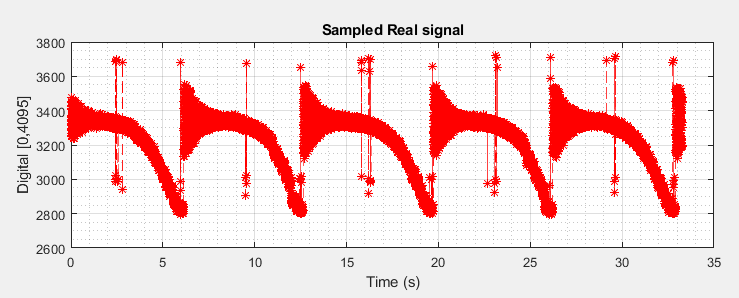
\includegraphics[width=0.7\linewidth]{ResistorReal2}
    \caption{Real component.}
    \label{fig:ResistorReal2}
\end{subfigure}
\begin{subfigure}{0.99\textwidth}
\centering
    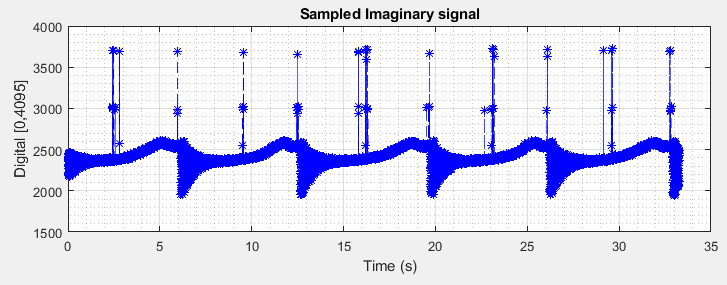
\includegraphics[width=0.7\linewidth]{ResistorImaginary2}
    \caption{Imaginary component.}
    \label{fig:ResistorImaginary2}
\end{subfigure}
\caption{Sampled signals in time at the ADCs, which represent the current response for the spectroscopy of a 9.95 k$\Omega$ discrete resistor.}
\label{fig:ResistorSignalsTime}
\end{figure}

The current responses of \autoref{fig:ResistorSignalsTime} are transformed into impedance magnitude and phase using \autoref{eq:CorrectedMagnitude} and \autoref{eq:CorrectedPhase}. All the impedance datapoints are represented as a function of frequency in \autoref{fig:ResistorImpedance}. \par
\begin{figure}[h]
\centering
\begin{subfigure}{0.99\textwidth}
\centering
    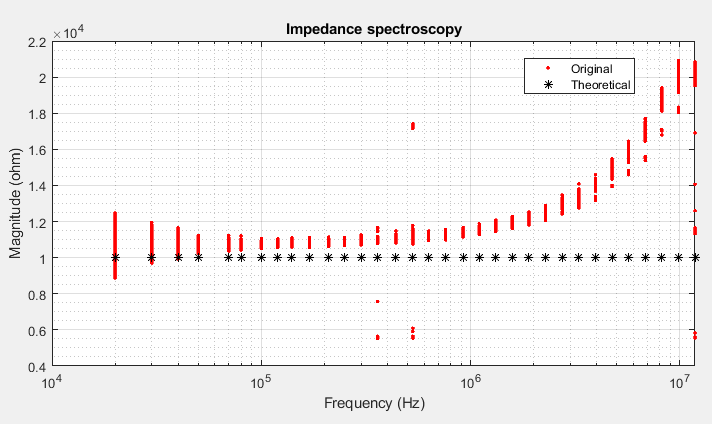
\includegraphics[width=0.9\linewidth]{ResistorMagnitude2}
    \caption{Magnitude.}
    \label{fig:ResistorMagnitude2}
\end{subfigure}
\begin{subfigure}{0.99\textwidth}
\centering
    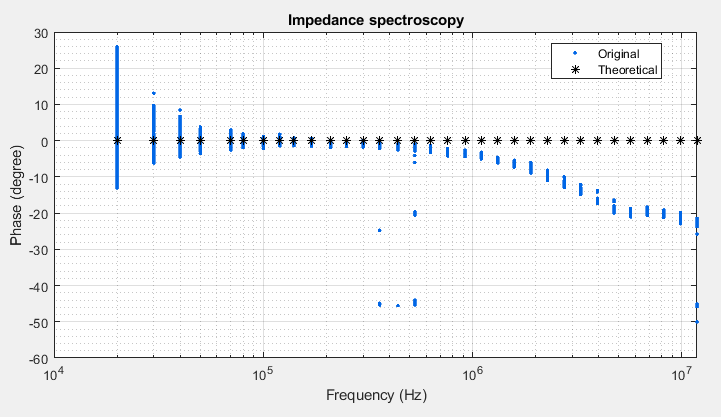
\includegraphics[width=0.9\linewidth]{ResistorPhase2}
    \caption{Phase.}
    \label{fig:ResistorPhase2}
\end{subfigure}
\caption{Bode plot of the sampled impedance of a 9.95 k$\Omega$ discrete resistor with its theoretical value.}
\label{fig:ResistorImpedance}
\end{figure}

Some outliers can be observed from that dataset, which are introduced by a fault in the sampling protocol of the MCU. These errors are only present for the multi-frequency mode and will be kept to show the robustness of the measurements to outliers. \par

The values for low frequency also present a large imprecision. This imprecision is to be expected since the impedance-sensing system is definded only for frequencies above 100kHz. The LPF of the PSDs thus have a -3dB low-pass frequency of 20kHz, which does not totally attenuates the signal up until at least 70 kHz. \par

A significant bias can be observed at high frequency, which orgininates from a couple of causes. Firstly, the op-amps used in the electronics of the numerous modules (see \autoref{chap:Electronics}) have a frequency limit defined by their slew-rates, input capacitance, and gain-bandwidth. Secondly, capacitive coupling is introduced because of the PCB dielectric, traces, and wires. Those tend to attenuate the high-frequency components of signals. Since square excitation signals are used, the harmonics at higher frequencies get attenuated until the signal behaves much more like a sinewave around 20 MHz. As a result, the perceived impedance from the impedance-sensing device is increased since the measured current response gets lower at high frequency (refer to \autoref{eq:Magnitude}). \par

To solve this issue and linearize the sensor, a calibration is realized using resistors of different values. Since the parasitics are singular to the electronics, the same nonlinearity will be found for different values of resistance, which can be used as a frequency-dependant factor to linearize the magnitude and phase curves. The results of such a calibration are shown in \autoref{fig:ResistorImpedanceCalibrated}. \par
\begin{figure}[h]
\centering
\begin{subfigure}{0.99\textwidth}
\centering
    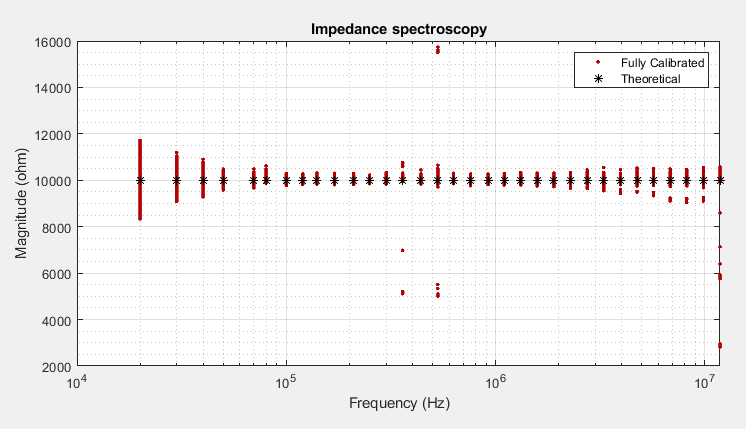
\includegraphics[width=0.9\linewidth]{ResistorMagnitudeCalibrated2}
    \caption{Magnitude.}
    \label{fig:ResistorMagnitudeCalibrated2}
\end{subfigure}
\begin{subfigure}{0.99\textwidth}
\centering
    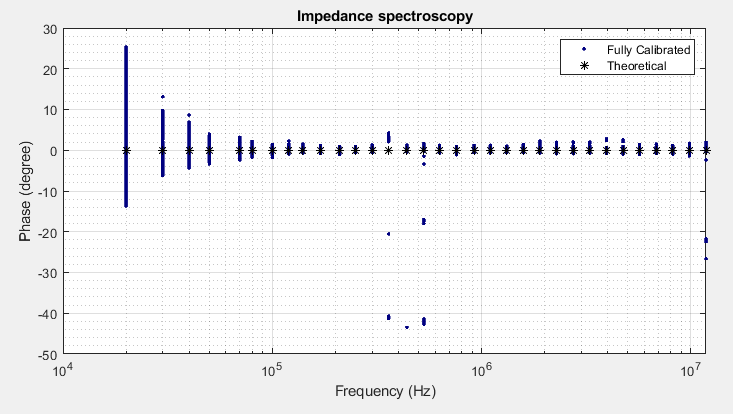
\includegraphics[width=0.9\linewidth]{ResistorPhaseCalibrated2}
    \caption{Phase.}
    \label{fig:ResistorPhaseCalibrated2}
\end{subfigure}
\caption{Bode plot of the calibrated impedance of a 9.95 k$\Omega$ discrete resistor with its theoretical value.}
\label{fig:ResistorImpedanceCalibrated}
\end{figure}

Since this situation is only in the Real realm (no imaginary values are observed after calibration), the square to sine conversion is not needed, as proved in \autoref{sec:ImpedancePrinciples}. 

Thus, from the previous curves, errors of less than 1.5\% for the magnitude and of less than 2.5\% for the phase are observed for all the frequencies considered in the spectroscopy. The system thus works as intended. \par


\subsection{Complex discrete model}
The same procedure can be repeated for a more complex discrete model. A 10 k$\Omega$ resistor is placed in series with the parallel combination of a 4.47 k$\Omega$ resistor and a 100 pF capacitor. The current response at the ADCs are transformed into impedance magnitude and phase using \autoref{eq:CorrectedMagnitude} and \autoref{eq:CorrectedPhase}, then calibrated the same way as for the discrete resistor of the last example. All the calibrated impedance datapoints are represented as a function of frequency in \autoref{fig:RCImpedanceCalibrated}. \par

The impedance curves are calibrated to get \autoref{fig:RCImpedanceCalibrated}. \par
\begin{figure}[h]
\centering
\begin{subfigure}{0.99\textwidth}
\centering
    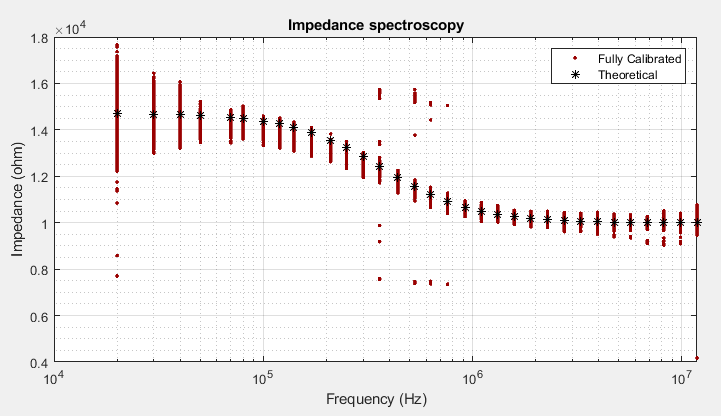
\includegraphics[width=0.9\linewidth]{RCMagnitudeCalibrated2}
    \caption{Magnitude.}
    \label{fig:RCMagnitudeCalibrated2}
\end{subfigure}
\begin{subfigure}{0.99\textwidth}
\centering
    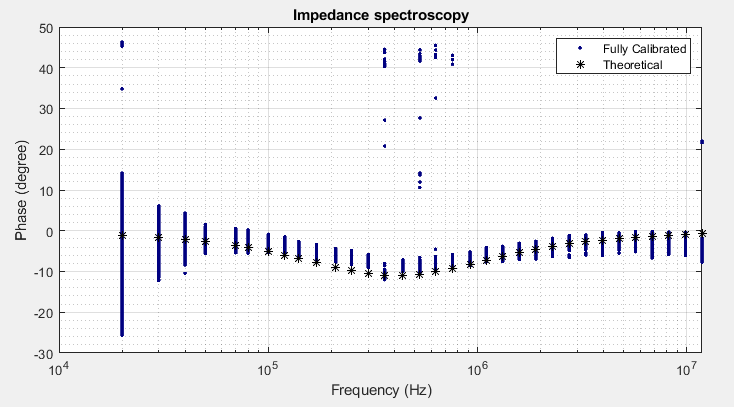
\includegraphics[width=0.9\linewidth]{RCPhaseCalibrated2}
    \caption{Phase.}
    \label{fig:RCPhaseCalibrated2}
\end{subfigure}
\caption{Bode plot of the calibrated impedance of a 10 k$\Omega$ discrete resistor in series with a parallel combination of a 4.47 k$\Omega$ resistor and a 100pF capacitor.}
\label{fig:RCImpedanceCalibrated}
\end{figure}

These follow adequately the theoretical curves, but a bias is still to be found. This bias can be solved using the square to sine conversion adapted from \citep{Subhan2019} and described in \autoref{sec:ImpedancePrinciples}. This conversion can not be used on such a large dataset as in \autoref{fig:ResistorImpedanceCalibrated}, only the median value of all the data taken at one frequency points will be considered henceforth to represent spectroscopy. The results of such a conversion are shown in \autoref{fig:RCImpedanceSine}. \par
\begin{figure}[h]
\centering
\begin{subfigure}{0.99\textwidth}
\centering
    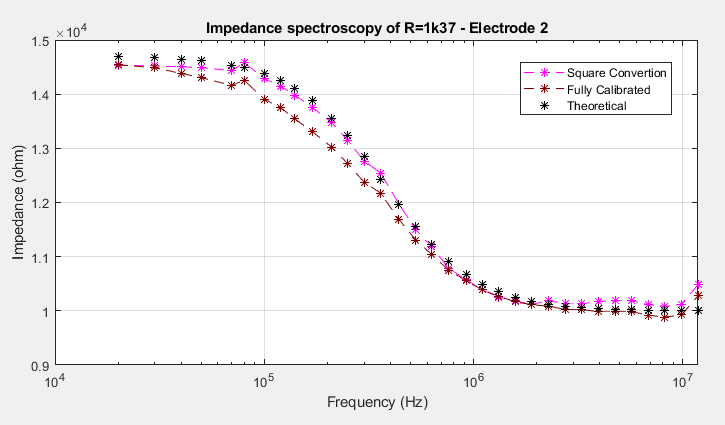
\includegraphics[width=0.9\linewidth]{RCMagnitudeSine2}
    \caption{Magnitude.}
    \label{fig:RCSineMagnitude2}
\end{subfigure}
\begin{subfigure}{0.99\textwidth}
\centering
    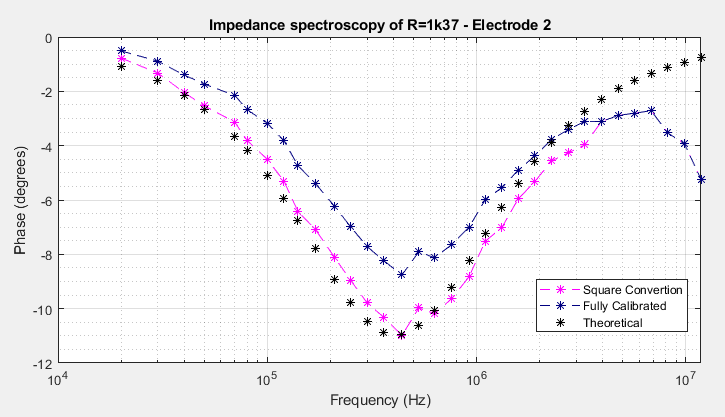
\includegraphics[width=0.9\linewidth]{RCPhaseSine2}
    \caption{Phase.}
    \label{fig:RCPhaseSine2}
\end{subfigure}
\caption{Bode plot of the calibrated impedance of a 10 k$\Omega$ discrete resistor in series with a parallel combination of a 4.47 k$\Omega$ resistor and a 100pF capacitor, after conversion from square to sine spectroscopy.}
\label{fig:RCImpedanceSine}
\end{figure}
At high frequencies, the square to sine conversion does not have enough datapoints to adequately do the conversion. This introduces a bias at high frequency. A way to solve this issue would be to extrapolate the behavior of the system from the previous points and use that extrapolation in the sqaure to sine conversion. For the case of simplicity in this study, no such correction shall be attempted.  \par

Apart from that, errors of less than 1.5\% for the magnitude and of less than 2.5\% for the phase are observed for all the frequencies considered in the spectroscopy. The system thus works as intended. \par